\section{Introduction}

\label{sec:intro}
The reconstruction of solid models from scattered point data is common and well studied problem in the field of computer graphics. Interest stems from the desire to convert real life data-sets acquired from range scanners to polygonal models. The idea also has applications in mesh cleaning (re-meshing or hole filling.) A common approach, given an oriented point set, is to find an implicit function such whose iso-surface corresponds to an approximation of the original surface.

In this work we apply the theory behind shift-invariant spaces (function spaces spanned by the lattice translates of a generating kernel) to the Poisson surface reconstruction problem. The extension to these function spaces allows us to choose non-Cartesian lattice sites to which we anchor our kernel functions (\SC{sec:smpl_review}). Although our approach is general and applicable to any shift-invariant spanned by sufficiently smooth basis functions, we are specifically interested in those defined over the \emph{Body Centered Cubic} (BCC) lattice. Our focus is on reconstructing an approximate indicator function (a function that evaluates to one inside the model, and zero outside) in optimal function spaces, arguing that the sub-optimality of Cartesian-like methodologies may impact the accuracy of reconstructed surfaces.

\begin{figure*}
  \centering
  \mbox{} \hfill
	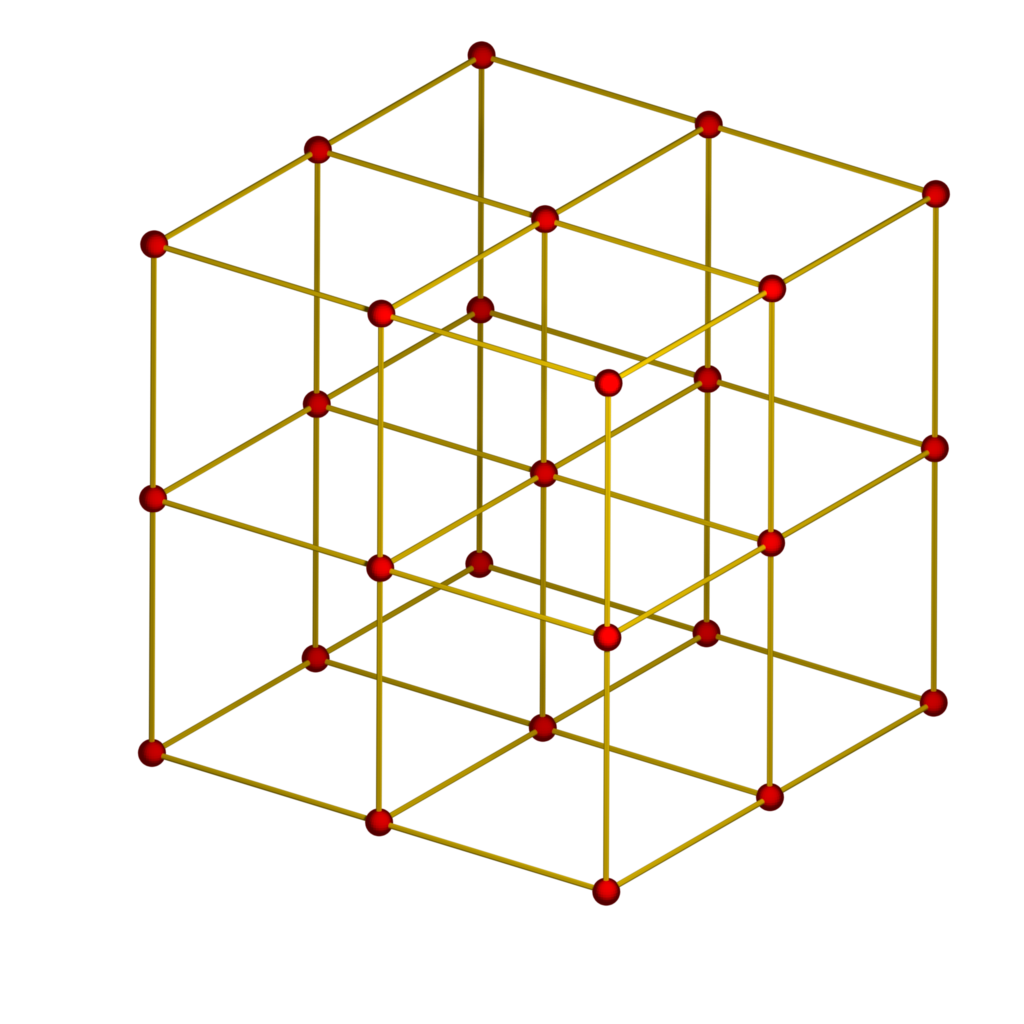
\includegraphics[width=.3\linewidth]{figures/lattice/cc}
	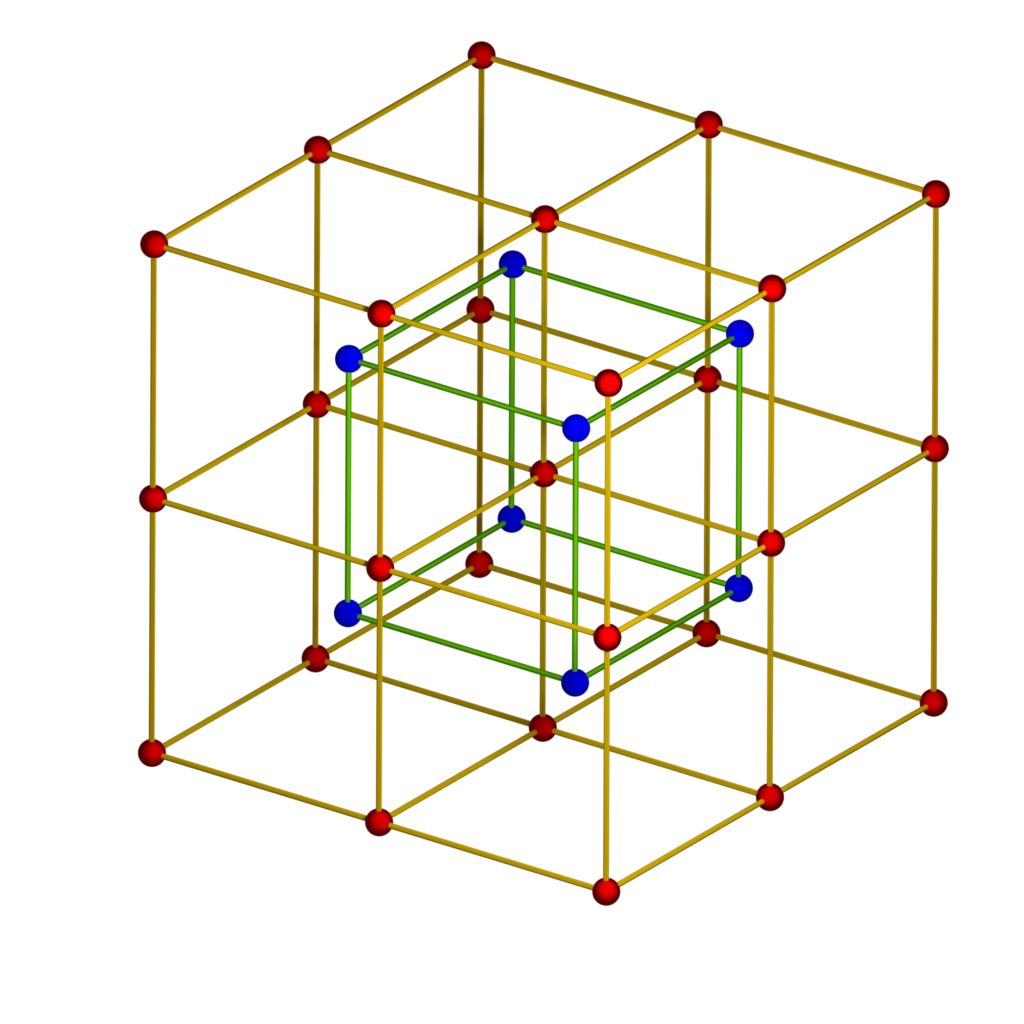
\includegraphics[width=.3\linewidth]{figures/lattice/bcc}
	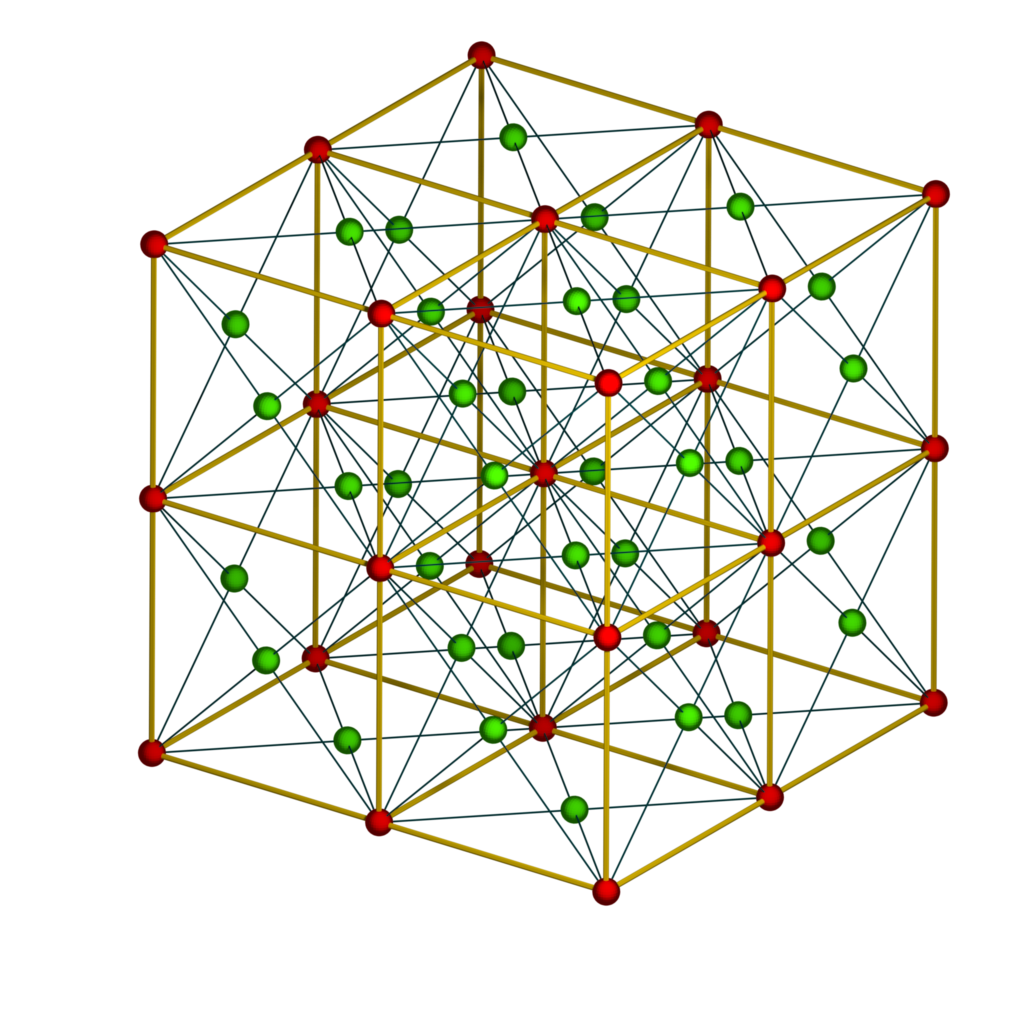
\includegraphics[width=.3\linewidth]{figures/lattice/fcc} \\
	
  \mbox{} \hfill
	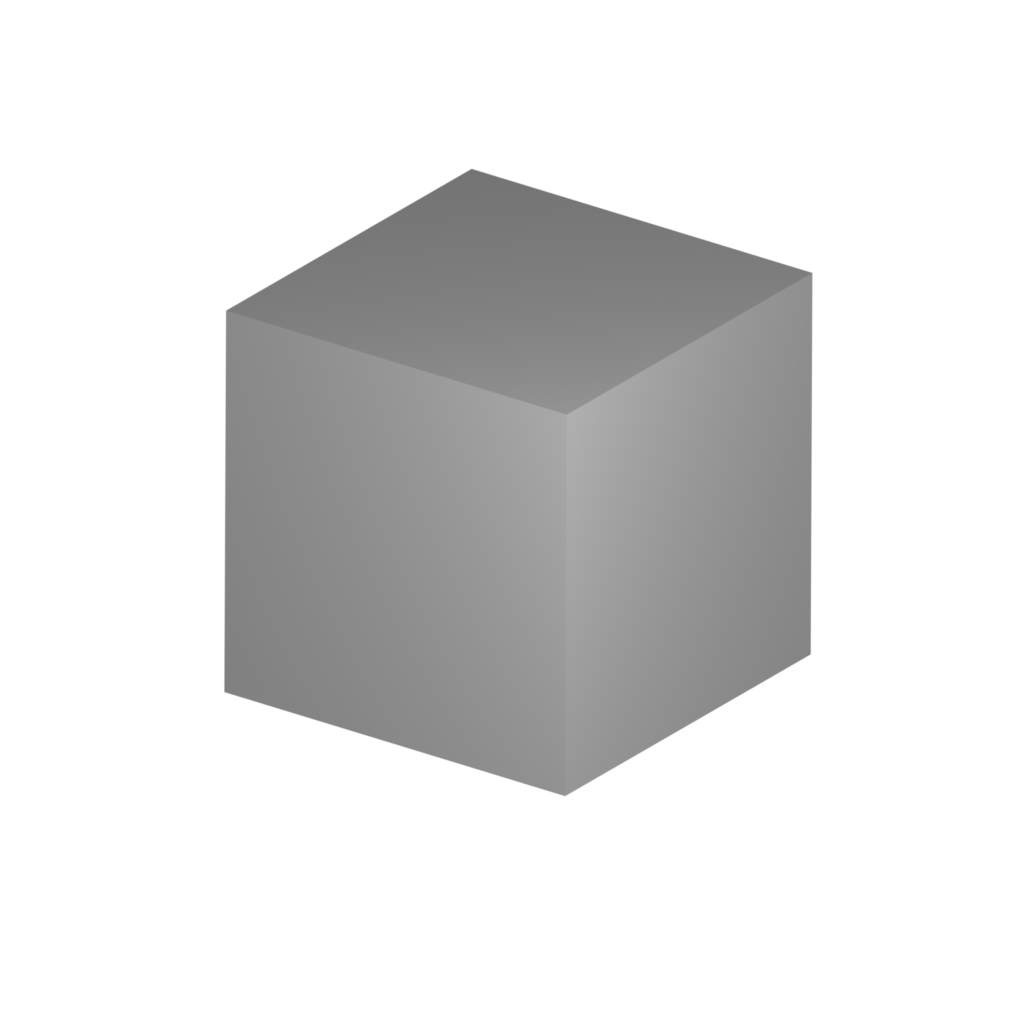
\includegraphics[width=.3\linewidth]{figures/lattice/cc_cell}
	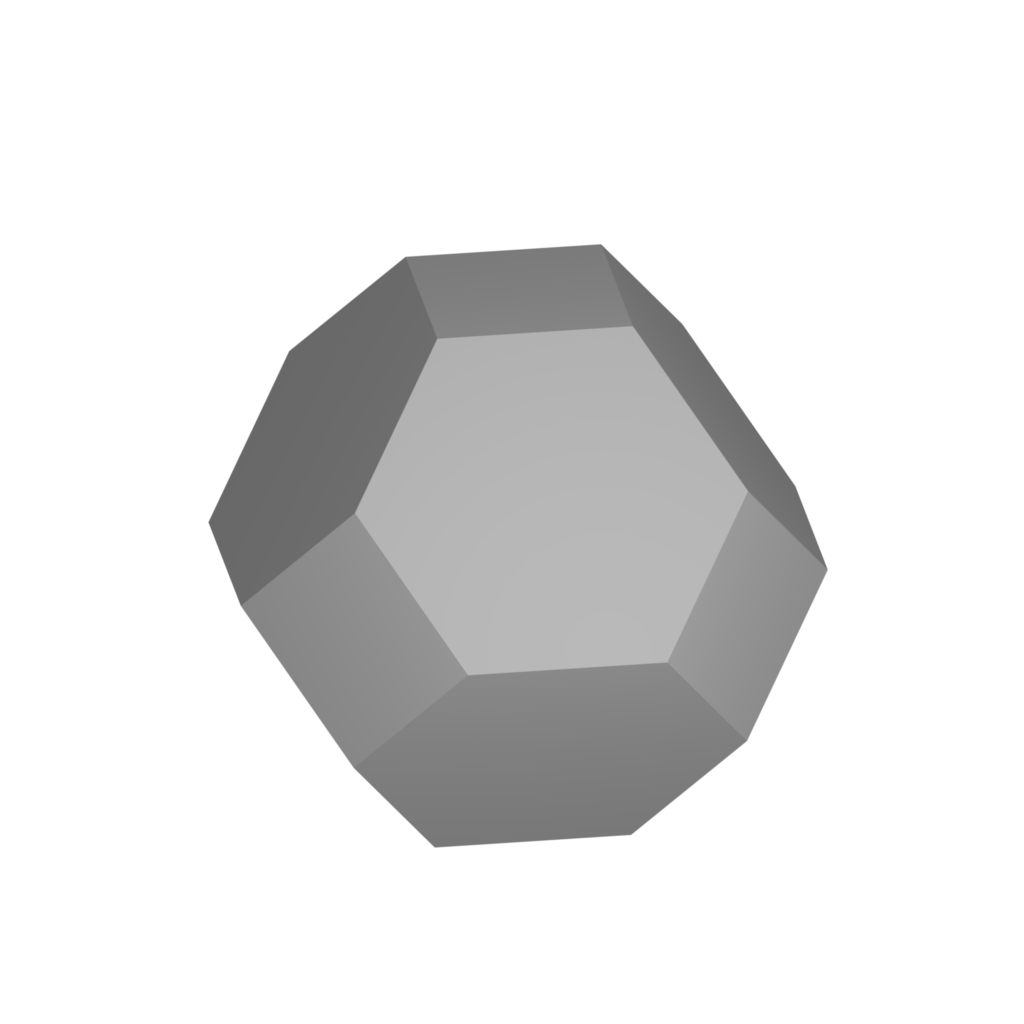
\includegraphics[width=.3\linewidth]{figures/lattice/bcc_cell}
	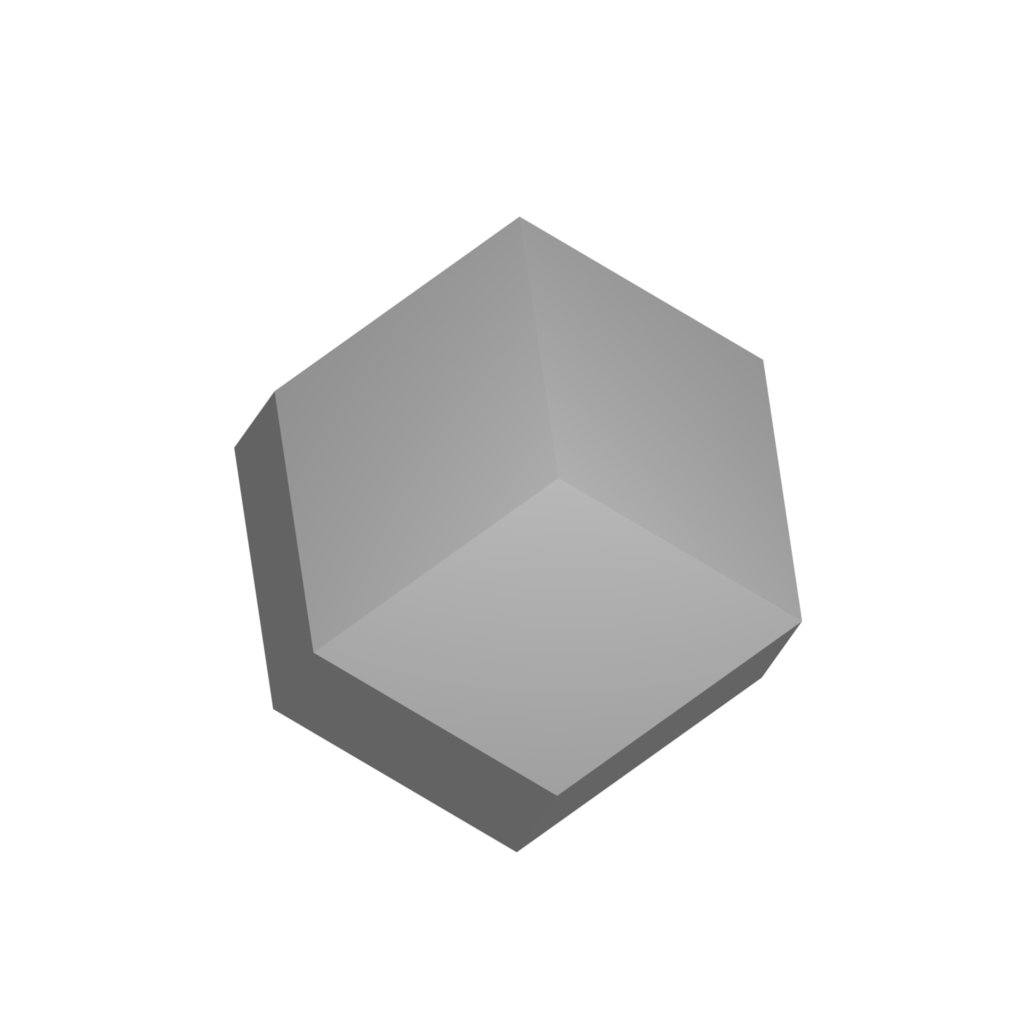
\includegraphics[width=.3\linewidth]{figures/lattice/fcc_cell} \\
   \hfill \mbox{}
  \caption{\label{fig:lattices}%
  Sampling lattices (top) with with their corresponding Voronoi regions (bottom). Left to right are the CC, BCC and FCC lattices respectively.
  }
\end{figure*}

The advantage of moving to the BCC lattice is two fold. First, it is well known that the BCC lattice generates the optimal sampling pattern in $\realn^3$. The argument for optimality is simple; a sampling of a function with respect to the BCC lattice is tantamount to a periodization of it's frequency spectrum about the BCC's dual lattice, the \emph{Face Centered Cubic} (FCC) lattice. Optimality follows from the observation that the FCC lattice represents the optimal sphere packing in three dimensions, that is, it packs frequency replica as tightly as possible, resulting in less \emph{pre-aliasing} from sampling. For isotropically band-limited functions, the tighter packing of frequency content allows for about 30\% more information to be captured when compared to samplings generated from the Cartesian lattice. Second, there exist reconstruction filters on the BCC lattice that outperform equivalent filters on the Cartesian lattice in terms of both speed and accuracy \cite{practicalbox} (in software implementations.) These filters are also more compact than their typical Cartesian counterparts. In the context of our surface reconstruction scheme, this gives rise to regularization matrices that are more sparse on the BCC lattice, and tend to provide faster convergence. 

Our surface reconstruction methodology follows the general Poisson
approach. First, we construct a smoothed approximation to the gradient
field of a model's indicator function. The divergence of the gradient
field is estimated and subsequently fed into a Poisson solver that
outputs the coefficients needed to approximate the smoothed indicator
function in a target shift invariant space. This Poisson solver is tailored to cater to the approximation power provided by each space \cite{}. However, our approach is novel in two notable ways. Firstly, we employ a variational scheme to obtain a lattice-based approximation of the gradient field. This
scheme depends only on the generating kernel of the target space and optimizes a functional that incorporates interpolation and smoothness constraints. Secondly, we utilize the theory behind shift-invariant spaces to seek discretizations of the divergence and Laplacian operators that are tailored to exploit the full approximation capabilities of the target space. 


Additionally, we also consider the possibility of approximating the
smoothed gradient field representation within function spaces that are
spanned by shifted versions of a single generating kernel. In the
context of gradient estimation, introducing a shift in the direction
of the derivative has shown to improve overall gradient
approximation fidelity in terms of gradient orientation and magnitude,
as well as displaying the ability to capture higher frequency details
that are smoothed out in non-shifted schemes~\cite{gradrev}. Since the
divergence operator is intimately connected to the gradient operator,
these results are of interest to us as using an appropriate
discretization of the derivative/divergence operator is an important facet
of recovering the indicator function of the initial model.

To summarize, our contributions are as follows:
\begin{itemize}
\item[$\bullet$] We cast the Poisson surface reconstruction problem
  into the framework of shift-invariant spaces.
\item[$\bullet$] Specifically, we investigate the reconstruction of
  surfaces in both a sub-optimal (Cartesian) and an optimal (BCC)
  box-spline function space.
\item[$\bullet$] We present a variational scheme that not only considers
  the usual centered generating kernels, but allows for the
  possibility of recovering each component of the gradient field in a
  space spanned by a shifted kernel. On the Cartesian
  lattice, these components are orthogonal whereas on the BCC lattice,
  the components are non-orthogonal and correspond to the directions
  associated with the underlying box-spline matrix.
\item[$\bullet$] While our focus is on comparing the surface reconstruction algorithm on both the CC and BCC lattices, we also provide qualitative and quantitative comparisons between the presented technique (on both the Cartesian and BCC lattices) and similar methods. 
\end{itemize}
